% Please use the skeleton file you have received in the 
% invitation-to-submit email, where your data are already
% filled in. Otherwise please make sure you insert your 
% data according to the instructions in PoSauthmanual.pdf
\documentclass{PoS}

\title{The $\gamma$-ray Milky Way above 10 GeV:\\
Distinguishing Sources from Diffuse Emission}

\ShortTitle{Distinguishing Sources from Diffuse Emission}

\author{\speaker{E. Owen},$^a$ C. Deil,$^{a}$ A. Donath,$^{a}$ R. Terrier$^{b}$\\
\llap{$^a$}Max-Planck-Institut f\"{u}r Kernphysik, P.O. Box 103980, D
69029 Heidelberg, Germany\\
\llap{$^b$}Astroparticule \& Cosmologie, CNRS, 75205 Paris Cedex 13, France\\
E-mail: \email{ellis.owen@mpi-hd.mpg.de}, \email{christoph.deil@mpi-hd.mpg.de}, \email{axel.donath@mpi-hd.mpg.de}, \email{terrier@apc.univ-paris7.fr}}


\abstract{One of the most prominent features of the $\gamma$-ray sky is the emission from our own Galaxy. The Galactic plane has been observed by \textit{Fermi}-LAT in GeV and H.E.S.S. in TeV light. Fermi has modeled the Galactic emission as the sum of a complex `diffuse' emission model with the predominately point source catalogs of 1FHL and 2FGL, while H.E.S.S. has primarily detected extended TeV sources. At GeV energies, Galactic diffuse emission dominates the $\gamma$-ray Milky Way but, as sources have hard spectra, it is likely their emission dominates at TeV energies. Generally the spatial shape and fraction of source emission compared to diffuse emission in the Galactic plane is not well known and is dependent on the source detection method, threshold and diffuse emission modeling methods used. \\

We present a simple image-analysis based method applied to \textit{Fermi}-LAT data from 10 GeV to 500 GeV, covering a region of +/- 5 degrees in Galactic latitude and +/- 100 degrees in Galactic longitude, to separate source and diffuse emission. This method involves elongated filter smoothing, combined with significance clipping to exclude sources. We test the method against models based on the 1FHL catalog and very simple model Galaxies to evaluate the response for an input of known fraction and shape of diffuse and source emission.}

\FullConference{Science with the New Generation of High Energy Gamma-ray experiments, 10th Workshop - Scineghe2014\\
		04-06 June 2014\\
		Lisbon - Portugal}
    
\usepackage{multirow}
\usepackage{gensymb}
\usepackage{wrapfig}
\usepackage{amsmath}
\usepackage{wasysym}
\usepackage{graphicx}
\usepackage{caption}
\usepackage{subcaption}
\usepackage{enumitem}
\DeclareGraphicsExtensions{.pdf}
\begin{document}

\section{Introduction}

In this work, we study the separation of sources from Galactic diffuse emission using image-based techniques. These are applied to data at energies between 10 and 500 GeV in order to understand appropriate methods for automatic diffuse modeling and source detection.

\begin{wrapfigure}{r}{0.55\textwidth}
\vspace{-10pt}
  \centering
      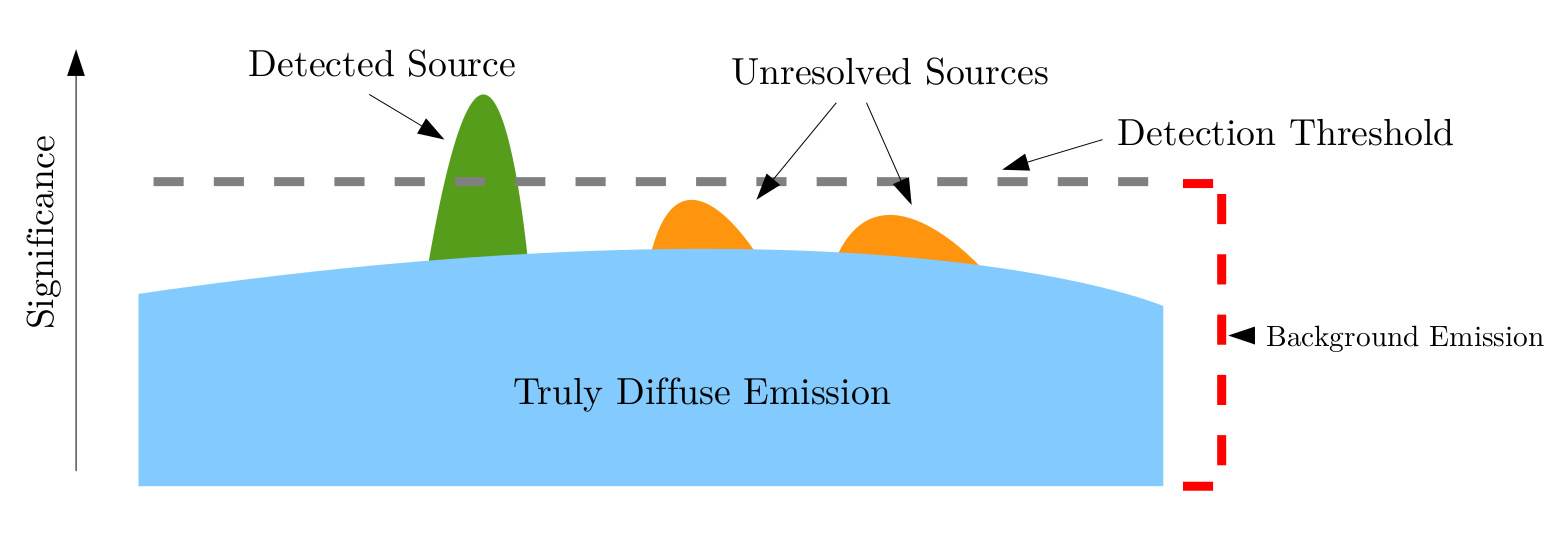
\includegraphics[width=0.55\textwidth]{figures/definitions.png}
  \caption{Galactic emission definitions.}
\vspace{-15pt}
\end{wrapfigure}

There is a need in the $\gamma$-ray astronomy community for a method of separating source and background `diffuse' emission in the Milky Way. In high-energy GeV and TeV data analysis, the challenge lies in finding methods that are suitable for use with the low statistics observed in order to provide reliable, stable results.

Galactic emission may be regarded as the sum of a number of distinct components. As definitions of these in the literature is non-standardized, we set here conventions for the terminology applied to this work. These definitions are illustrated in Figure 1.

\begin{itemize}[noitemsep,nolistsep]
\item \textbf{Sources} are to resolvable sources of $\gamma$-rays above a given instrument detection threshold.
\item \textbf{Unresolved sources} are those sources which physically exist but fall below the detection threshold of a given instrument, and so are not distinguished.
\item \textbf{Truly diffuse Galactic emission} refers to the flux contribution from physical processes leading to diffuse cosmic ray emission - at TeV energies, this is dominated by inverse Compton and $\pi^0$ decay while at lower GeV energies bremsstrahlung also contributes significantly.
\item \textbf{Galactic background emission} is the Galactic flux contribution which cannot be directly attributed to sources. As such, this is considered as the sum of the unresolved and truly diffuse emission contributions. In this work, this Galactic background emission is referred to as `diffuse' emission.
\end{itemize}

\section{Method}

An algorithm based on convolution with an elongated background filter and significance clipping is introduced. The operation of the algorithm is summarized in the following steps.

\begin{itemize}[noitemsep,nolistsep]
\item \textbf{Background:} Convolution of a counts map with a background kernel to act as an initial diffuse estimation.
\item \textbf{Significance:} A significance image is computed from the counts map and diffuse estimation image.
\item \textbf{Mask image computation:} From the significance image, an exclusion mask is determined, removing regions above a set significance threshold. These regions are replaced with a diffuse estimation based on the flux around the excluded source within a background convolution kernel. The significance and mask image computation steps repeat, with excluded regions dilated in each iteration for which they fall above the significance threshold. Once there is no change in the exclusion mask, the final diffuse estimation image is returned.
\end{itemize}

The method is specified by the six parameters indicated in Table 2, p. 5 (the values indicated refer to the example application to the dataset discussed in sections 3 and 4), and can be considered as a generalization of the ring background method \cite{berge} adapted to handle elongated diffuse estimation in the Galactic plane through the use of an lengthened background kernel.

The initial diffuse estimation is taken as the total flux contribution, as determined from the provided counts image. From this, the mask grows with each iteration around significantly detected sources, leading to the gradual reduction in the estimated diffuse flux with each iteration.

In such instances, the resulting diffuse estimation algorithm will either fail, or the results should not be trusted. Primarily, in cases for which the background kernel is too small, there will be regions around sources where the exclusion mask dilates to a size larger than the box, hence diffuse estimation will fail since there is no remaining data within the kernel from which a diffuse estimate can be determined. Additionally, in cases of very low counts ($\approx \mathcal{O}(10)$ events in the background kernel) the results are dominated by Poisson fluctuations such that any diffuse estimate would not be reliable. In these cases, it may be found that the algorithm fails completely due to an inability to determine significance values for the full analysis region, or returns a null result.

\section{Dataset}

The datasets upon which the method is demonstrated comprise both of experimental observations and simulated inputs intended to provide a realistic and well-understood test-base. Both are described in this section.

For all datasets, an analysis region of Galactic latitude $-5 < b < 5$ $deg$ and longitude $-100 < l < 100$ $deg$ is used to encompass the majority of the observed Galactic emission. This ensures regions of high source density around the Galactic center are included as well as offering variation in the population distribution at higher longitudes for a broad base of test cases.


\subsection{\textit{Fermi}-LAT}

\textit{Fermi}-LAT data from 5 years of observation was chosen with a well defined 10-500 GeV energy cut as a showcase for the method. This choice was due to a well-understood PSF, good coverage of the Galactic plane and roughly uniform exposure of the Galactic region of interest at these high energies. It should be noted that applications of this method in analyses need not be limited to \textit{Fermi}-LAT data: image analysis of all high-energy Galactic data is the intended use-case.

The available statistics for the energy range in question fall off steeply towards the higher end of the cut (for the Galactic region of interest, there are $6.2 \times 10^4$ events in the 10-500 GeV range, following a power-law of index $-1.55$). As such, there are suitable numbers of events for such an analysis to be undertaken on the dataset across the full energy band, but insufficient counts for a finer energy binning to be used.

\subsection{Simulation}

The simulated dataset may be split twofold. In both cases, a well-understood simple source population is added to a known diffuse contribution. In this case, the Fermi diffuse background model \verb|gll_iem_v05_rev1.fit| was taken.

The simulated inputs differ in that one uses a source contribution taken as a PSF-convolved point source image of the 1FHL catalog above 10 GeV, while the remaining three use entirely simulated Galactic source populations.

For the PSF convolved 1FHL catalog input, the resulting source-only image had a flux of $2.84\times 10^{-9} \text{ph cm}^{-2}\text{s}^{-1}$.

Where the source flux contribution was entirely simulated by model galaxies, the inputs were based on the study undertaken in the simulation work of the 1FHL Catalog paper \cite[p.59]{1fhl}, which followed the essence of the study presented in \cite{Strong}. This considered a reference galaxy of a similar source population and distribution to the Milky Way, and two further simulations with different densities and proportions of bright and faint sources.

In line with \cite{Strong}, it is assumed that the luminosity function of the $\gamma$-ray source population between two limits $L_{\gamma, min}$ and $L_{\gamma, max}$ follows a simple power law. Further, it is taken that the spatial distribution of pulsars offers representative example of spatial distribution of a Galactic $\gamma$-ray source population \cite[p.2]{Strong}. Thus we use a galactocentric $(R, z)$ pulsar distribution model \cite[p.7]{Lorimer} (a Gamma function) to distribute sources for the $\rho(R)$ radial source density distribution, and an exponential function for the $\rho(z)$ distribution. Standard Monte-Carlo methods are used to sample $\rho(L_{\gamma}, R, z)$ throughout the simulated galaxy. The resulting distribution is then normalized and scaled at $R_{\astrosun}$ to the observed population density at the Sun. In line with the 1FHL study, the radial distribution peaks at 4 kpc and the $\rho(z)$ exponential scale is set to 0.5 kpc.

A reference model (A) is defined with $\rho_{\astrosun} = 3 \text{kpc}^{-3}$, minimum $\gamma$ luminosity $L_{\gamma, min} = 10^{34} \text{ph s}^{-1}$ and maximum $\gamma$ luminosity $L_{\gamma, max} = 10^{37} \text{ph s}^{-1}$ with luminosity power-law index of $\Gamma=-1.5$. Two comparison models, B and C - both of higher population densities at the position of the Sun and lower luminosity bounds - are also considered. These are outlined in Table 3.

\begin{table}
\centering
\resizebox{\textwidth}{!}{
\begin{tabular}{|c|c|c|c|}
\hline
\multirow{ 2}{*}{\textbf{Source Model}} & \textbf{Population Density} & \textbf{Minimum Luminosity/} & \textbf{Maximum Luminosity/}\\
 & \textbf{at the Sun/$\text{kpc}^{-3}$} & \textbf{10$^{33} \text{ph s}^{-1}$} & \textbf{10$^{36} \text{ph s}^{-1}$}\\\hline
A & 3 & 10 & 10 \\\hline
B & 10 & 4.0 & 4.0 \\\hline
C & 30 & 1.5 & 1.5 \\\hline
\end{tabular}}
\caption{Parameters for 10 - 500 GeV Galaxy Population Simulations.}
\end{table}

\begin{wrapfigure}{l}{0.4\textwidth}
\resizebox{0.4\textwidth}{!}{
\begin{tabular}{|c|c|}
\hline
\multirow{ 3}{*}{\textbf{Source Model}} & \textbf{Source Flux in} \\ 
 & \textbf{Galactic Region/}\\
 & \textbf{10$^{-8}$ ph cm$^{-2}$ s$^{-1}$}\\\hline
1FHL Catalog Sources & 0.28 \\\hline
A & 1.70 \\\hline
B & 1.94 \\\hline
C & 1.99 \\\hline
\end{tabular}}
\makeatletter
\def\@captype{table}
\makeatother
\caption{Simulated source fluxes}
\vspace{-30pt}
\end{wrapfigure}

Before application to the source separation algorithm, the 1FHL and simulated catalogs are added to the integrated Fermi Diffuse background model \verb|gll_iem_v05_rev1.fit| between 10 GeV and 500 GeV to produce the input source \& diffuse test cases. The integral flux of this model in the Galactic plane region was $2.85 \times 10^{-7} \text{ph cm}^{-2}\text{s}^{-1}$. The fluxes of the four source populations are given in Table 2.

\newpage
\section{Results}

In application to these inputs, the parameters for the algorithm were specified as per Table 3. The significance threshold was set through preliminary studies to understand how to avoid significance-triggering (and hence false source detection) on Poisson up-fluctuations. This was achieved by Poisson-fluctuating a uniform input image and selecting a significance threshold above that for which false detections were avoided. The correlation radius and mask dilation radius were chosen to be of the order of the \textit{Fermi}-LAT PSF to optimize for point source detection (the LAT PSF has a 68 \% containment radius of 0.150 $deg$ and 95 \% containment radius of 0.867 $deg$ in the 10-500 GeV energy band), while an elongated background kernel of suitable size to ensure all exclusion regions could be covered. A pixel size of 0.1 $deg$ in each dimension offered good resolution for source detection without leading to an excessive computational load during analysis.

\begin{wrapfigure}{r}{0.5\textwidth}
\vspace{-10pt}
\begin{center}
\begin{tabular}{|c|c|}
\hline
\textbf{Parameter} & \textbf{Value}\\\hline
Significance cut off & 4 $\sigma$\\\hline
Correlation radius & 0.3\degree \\\hline
Mask dilation radius & 0.3\degree \\\hline
Height of background kernel & 0.5\degree \\\hline
Width of background kernel & 10\degree \\\hline
Pixel size & 0.1\degree \\\hline
\end{tabular}
\end{center}
\makeatletter
\def\@captype{table}
\makeatother
\caption{Separation Algorithm Parameters}
\vspace{-20pt}
\end{wrapfigure}

The results from simulated galaxy models are given in Table 4, summarizing the total diffuse flux in the Galactic region and the recovered source flux determined by the algorithm compared to the input true source flux fraction. These results indicate that this method offers best performance in cases where the source population density is lower and is comprised of more luminous sources. In diffuse estimation, the method is less able to successfully resolve and remove lower luminosity source populations since a greater proportion fall below a detection threshold. Additionally, higher density populations where clustered sources may be confused with an extended diffuse morphology also lead to less successful separation results.

\begin{table}
\centering
\resizebox{\textwidth}{!}{
\begin{tabular}{|c|c|c|c|}
\hline
\textbf{Source Model} & \textbf{Separated Background Flux/} & \textbf{True Source} & \textbf{Recovered Source}\\
\textbf{(\& Fermi Diffuse Background)} & \textbf{10$^{-7}$ ph cm$^{-2}$ s$^{-1}$} & \textbf{Flux Fraction/\%} & \textbf{Flux Fraction/\%}\\\hline
Fermi 1FHL Catalog > 10 GeV & 2.8 & 0.99 & 1.4\\\hline
Reference Simulation & 2.9 & 5.6 & 3.6\\\hline
Simulation 1 & 3.0 & 6.4 & 2.3\\\hline
Simulation 2 & 3.0 & 6.5 & 2.0\\\hline
\end{tabular}}
\makeatletter
\def\@captype{table}
\makeatother
\caption{Galactic Plane recovered diffuse fluxes}
\end{table}

Application to true \textit{Fermi}-LAT data to develop a diffuse model (Figure 3) produced a diffuse estimation with a flux of $9.90 \times 10^{-8}$ ph cm$^{-2}$ s$^{-1}$ in the Galactic region. Figure 4 presents spatial profiles of the resulting diffuse model. It can be seen that the diffuse estimation here largely follows the total flux distribution of the Milky Way, with some sources excluded. Shortcomings are evident where diffuse estimation exceeds the total flux. This arises due to an inappropriately large size of the background convolution kernel in such regions, combined with source contamination in the diffuse estimation. Improved results may be possible with fine-tuning of algorithm parameters and multiple iterations of varying convolution kernel sizes which would better account for more of the extended source population.

\begin{figure}
  \begin{center}
      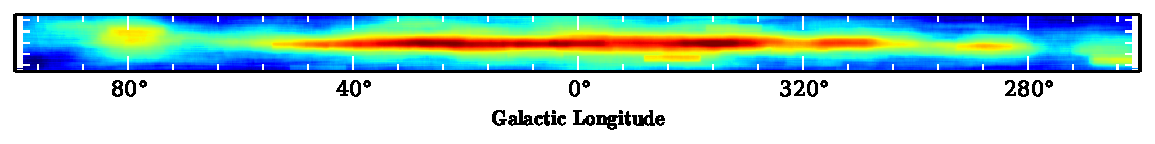
\includegraphics[width=\textwidth]{figures/BG_DATA.pdf}
  \caption{Background estimation for \textit{Fermi}-LAT Data.}
  \end{center}
\end{figure}

\begin{figure}
\centering
\begin{subfigure}{0.33\textwidth}
      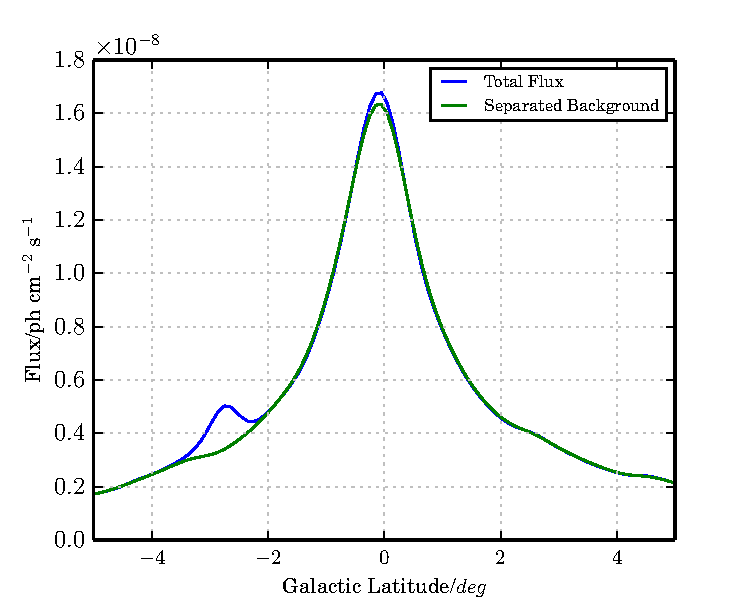
\includegraphics[width=\textwidth]{figures/GLAT.pdf}
\end{subfigure}
\begin{subfigure}{0.66\textwidth}
        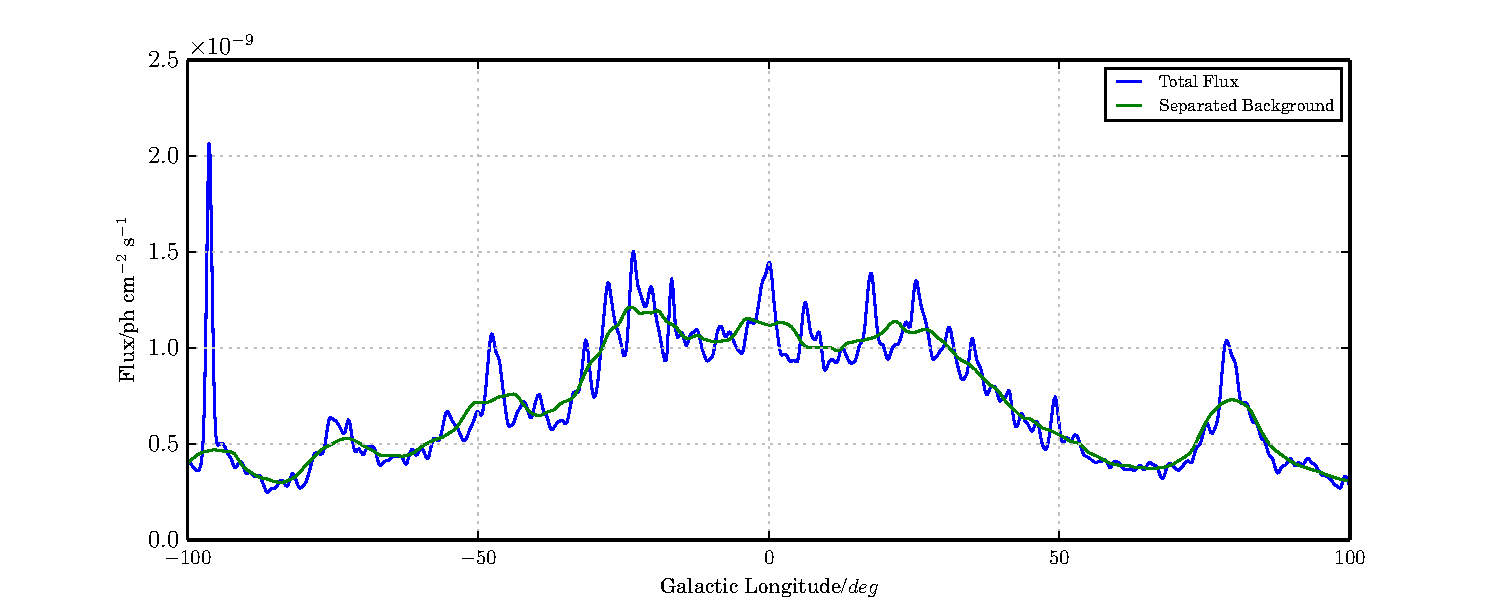
\includegraphics[width=\textwidth]{figures/GLON.pdf}
\end{subfigure}
\caption{\textit{Fermi}-LAT Profiles for total Galactic flux and estimated diffuse flux}
\end{figure}

\section{Conclusions}

We present a method of modeling the Galactic diffuse emission and test against simulated Galaxies with reasonable results. Application to observational data offers a realistic diffuse model of similar flux levels to those seen in the Fermi Diffuse Model \verb|gll_iem_v05_rev1.fit|.

Some weaknesses of the method can be seen in the overestimation of the diffuse flux contribution in some regions. Steps are suggested for fine-tuning which, combined with algorithm extensions to allow for iterative application of multiple background kernels, may improve the diffuse estimation.

The methods and algorithm introduced in this study, including the Galaxy simulation methods, are provided in the affiliated Astropy open-source Python package, Gammapy \cite{Deil}.

\begin{thebibliography}{99}

\bibitem{berge}
D.~Berge, S.~Funk and J.~Hinton.
\newblock {B}ackground {M}odelling in {V}ery-{H}igh-{E}nergy $\gamma$-ray {A}stronomy.
\newblock In {\em {A}stronomy \& {A}strophysics}, 466(3):1219, 2008.

\bibitem{Deil}
C.~Deil, A.~Donath, E.~Owen, R.~Terrier and R.~B{\"{u}}hler.
\newblock {G}ammapy {0.1}: {G}amma-ray astronomy with {P}ython.
\newblock In {\em {P}roceedings of the {S}eventh {E}uropean {C}onference on
  {P}ython in {S}cience (in preparation)}.
\newblock Software available online: {\verb|https://github.com/gammapy/gammapy|}.

\bibitem{1fhl}
{The Fermi-LAT Collaboration}.
\newblock The {F}irst {Fermi-LAT} {C}atalog of {S}ources {A}bove 10 {GeV}.
\newblock {\em Astrophysical Journal Supplement Series}, 209(2):34, 2013.

\bibitem{Lorimer}
D.~R. Lorimer.
\newblock {T}he {P}arkes multibeam pulsar survey: {VI.} {D}iscovery and timing
  of 142 pulsars and a {G}alactic population analysis.
\newblock {\em Monthly Notices of the Royal Astronomical Society}, 372(2):777,
  2006.

\bibitem{Strong}
A.~W. Strong.
\newblock {S}ource population synthesis and the {G}alactic diffuse gamma-ray
  emission.
\newblock {\em Astrophysics and Space Science}, 309, 2007.


\end{thebibliography}
\end{document}


